\documentclass[letterpaper, 10pt, conference]{ieeeconf}

\usepackage{xspace}
\usepackage{graphicx}
\usepackage{multirow}
\usepackage{booktabs}
\usepackage{numprint}
\usepackage{acro}
\setlength {\marginparwidth}{2cm}
\usepackage{todonotes}
\setuptodonotes{inline}

\usepackage{acro}

% workaround for
% https://bitbucket.org/cgnieder/acro/issues/120/having-an-acronym-in-plural-form-the-first
\let\IDeclareAcronym\DeclareAcronym
\renewcommand{\DeclareAcronym}[2]{%
  \IDeclareAcronym{#1}{%
    #2,foreign-plural={}
  }
}

\DeclareAcronym{rrt}{
  short = RRT$^*$,
  long = Rapidly-exploring Random Tree
}

\DeclareAcronym{ara}{
  short = ARA$^*$,
  long = Anytime Repairing A$^*$
}

\DeclareAcronym{plrrt}{
  short = PL-RRT$^*$,
  long = Path Length Rapidly-exploring Random Tree
}

\DeclareAcronym{plara}{
  short = PL-ARA$^*$,
  long = Path Length Anytime Repairing A$^*$
}

\DeclareAcronym{mcrrt}{
  short = MC-RRT$^*$,
  long = Motion Cost Rapidly-exploring Random Tree
}

\DeclareAcronym{mcara}{
  short = MC-ARA$^*$,
  long = Motion Cost Anytime Repairing A$^*$
}

\DeclareAcronym{knn}{
  short = $k$-NN,
  long = $k$-nearest neighbors,
}


\newcommand{\E}[0]{Euclidean\xspace}
\newcommand{\D}[0]{Dubins\xspace}
\newcommand{\DF}[0]{Dubins~+~Filter\xspace}

\IEEEoverridecommandlockouts
\overrideIEEEmargins

\title{\LARGE \bf
  Planning for Air Traffic Control*
}

\author{Ben Potter$^{1}$
  \thanks{
    *This work was completed for ELEC 844 taught
    by Jonathan Gammell
  }
  \thanks{$^{1}$
    Department of Electrical and Computer Engineering,
    Queen's University,
    Kingston,
    Canada
    {\tt\small ben.potter@queensu.ca}
  }
}

\begin{document}

\maketitle
\thispagestyle{empty}
\pagestyle{empty}

\begin{abstract}
  This is an abstract.
\end{abstract}

\section{INTRODUCTION}

\begin{itemize}
  \item what is the problem
  \item why is it challenging
  \item use a sampling based planner because there are no narrow passages
  \item paper structure
\end{itemize}

\cite{tolstaya_rkk:planning_atc}

\section{BACKGROUND}

\begin{itemize}
  \item Dubins airplane
  \item Heuristic
  \item fixed-time motion primitives
\end{itemize}

\section{METHODOLOGY}

\begin{itemize}
  \item posit that it is true that if two states can be connected
    (according to the motion constraints) then as their euclidean
    distance decreases it looks identical to the dubins distance
\end{itemize}

\subsection{Anytime Repairing A$^*$}

\begin{itemize}
  \item how does ara work
  \item dynamic construction of grid
  \item goal region
\end{itemize}

\subsection{Rapidly-exploring Random Tree}

\begin{itemize}
  \item how does rrt work (more)
  \item how do we steer?
  \item how do we connect? if the states can be connected with constraints
  \item how does knn work?
  \item goal sampling
  \item Bounds on the search space
\end{itemize}

\ac{rrt} does not collapse to just finding the optimal Dubins path
between the start and the goal because these two states may not be
directly traversable in one step due to the kinodynamic constraints.

\todo{Define the Dubins airplane shortest cost path: cost of the path
  is referred to as the Dubins distance whereas the path itself is
called the Dubins path}

After a new state is added to the tree, I check whether the cost to
the \ac{knn} would improve through the new state.

The method of computing the \ac{knn} has a significant
impact on the performance of \ac{rrt}.
The \ac{knn} are computed multiple times in a single
iteration which has an large effect on runtime.
As the number of states in the tree grows, the algorithm must
spend more time computing distances.
The \ac{knn} are also used when perfoming local
optimization around a new state.
In this way, the algorithm has a direct impact on which states get
considered for rewiring.

I test three different distance metrics with \ac{knn}
that are based on the euclidean distance and the Dubins distance.
The \emph{\E} metric ranks states by their euclidean
distance which ignores the kinodynamic constraints of the airplane.
This approach dilutes the effect of local optimization by
underestimating the true distance between neighbors.
However, the euclidean distance is fast to compute which means
\ac{rrt} can spend more time searching.
Alternatively, the \emph{\D} metric computes the length of the
shortest path that obeys the kinodynamic constraints of the airplane
between neighbors.
This approach is slower to compute than the euclidean distance.
The Dubins distance, unlike the euclidean distance, is not
commutative (i.e., the Dubins distance from $a$ to $b$ is
not always the same as the Dubins distance from $b$ to $a$).
This requires computing the \ac{knn} for the candidate parents and
candidate children of each new state separately.
Finally, I consider a combination of these metrics called \emph{\DF}
where by the fast to compute euclidean distance is used to filter the
search tree down to the closest $2k$ states, before the Dubins distance
selects the best $k$ states.
This metric aims to use the speed of the \E metric while maintaining
the tight bound provided by the \D metric.

\begin{figure}[tbp]
  \includegraphics[width=\columnwidth]{figs/knn_benchmarks}
  \caption{}
  \label{fig:knn_benchmarks}
\end{figure}

I compare the performance of \ac{rrt} using different k-nearest neighbor
metrics in Fig.~\ref{fig:knn_benchmarks}.
As a measure of performance, I consider the number of iterations that
\ac{rrt} completes per millisecond which is shown on the y-axis.
The y-axis is shown in log scale.
I show how this metric changes as the number of states in the
search tree increases which is shown on the x-axis.
Each execution of \ac{rrt} is given the same start and goal states and
performs \numprint{10000} iterations.
The \DF metric seems to provide a runtime comparable to the \E
metric, even as the number of states grows large, while maintaining
the tight bound of the \D metric.
In the remaining results of this paper, I use the \DF metric to find
the \ac{knn} in \ac{rrt}.

\todo{mention kd tree}

\subsection{Motion Cost}

The penalty factor is learned from human guided trajectories.
We want the penalty to add a term to the cost function the planner uses.
In summary, the penalty is a number between 0 and 1.
We incorporate the penalty into the cost function by adding an
additional term which is the product of the penalty and the path length
through which that penalty is incurred.
If the penalty is 1, then the cost to reach the next state is
effectively double the path length.

I learn the penalty factor by recording a count of the number of times
that a human guided trajectory passes through each state.
As I want the penalty of a state to be lower when human guided
trajectories pass through that state more frequently, I invert this
count by taking the difference between the maximum count and the
count of each state.
Then, I normalize the counts so they fall between 0 and 1.

\begin{figure}
  \centering
  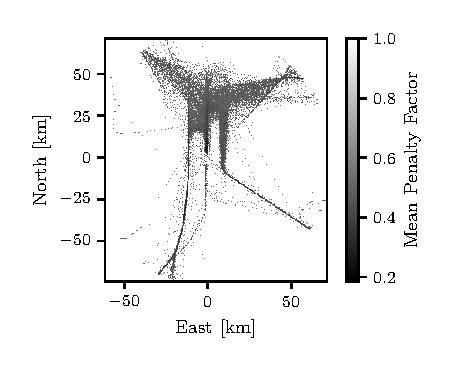
\includegraphics[width=\columnwidth]{figs/penalty}
  \caption{}
  \label{fig:penalty}
\end{figure}

\todo{Introduce the idea of Path Length versus Motion Cost}
\ac{plrrt}
\ac{mcrrt}
\ac{plara}
\ac{mcara}

Weighted sampling for RRT based on penalty
\begin{itemize}
  \item Tried rejection sampling but it didn't work because the low
    penalty regions are small compared to the sampling space which
    meant we spent too much time trying to randomly sample inside it
\end{itemize}

\subsection{Experiments}

\begin{itemize}
  \item what am i measuring
  \item path length (euclid for ara, dubins for rrt)
  \item number of iters
  \item number of states
  \item \textbf{how am i measuring it}
  \item What computer specs do I use?
  \item Describe HPC
  \item Describe gnu parallel \cite{tange:parallel}
\end{itemize}

\todo{Explain how the results were collected}

\section{DATASET PROCESSING}
\begin{itemize}
  \item Size around airport
  \item Days Jan 11, 12, 13, 14
  \item Arrivals at SEA
  \item Goal region?
  \item Wgs84 to ENU
  \item figure for the human trajectories
  \item Bearings
  \item Initial and final states
  \item path length (dubins and euclid)
\end{itemize}

\section{RESULTS}

\begin{table*}[!t]
  \renewcommand{\arraystretch}{1.3}
  \caption{}
  \label{tab:results}
  \centering
  \begin{tabular}{lllll}
    \hline
    \bfseries Planner & \bfseries Runtime [s] & \bfseries Median
    Iterations & \bfseries Median States & \bfseries Median Path Length \\
    \hline
    \multirow{3}{*}{\acs{plara}} & 30 & \numprint{504833.5} &
    \numprint{2415568.5} & \numprint{341.0} \\
    & 60 & \numprint{744918.5} & \numprint{3449428.5} & \numprint{335.5} \\
    & 180 & \numprint{1364171.5} & \numprint{5970043.5} & \numprint{315.5} \\
    \hline
    \multirow{3}{*}{\acs{plrrt}} & 30 & \numprint{53000.0} &
    \numprint{47694.0} & \numprint{81.9} \\
    & 60 & \numprint{79000.0} & \numprint{71092.0} & \numprint{81.9} \\
    & 180 & \numprint{136000.0} & \numprint{122535.0} & \numprint{81.9} \\
    \hline
    Human & & & & \numprint{111.3} \\
    \hline
    \hline
    \bfseries Planner & \bfseries Runtime [s] & \bfseries Median
    Iterations & \bfseries Median States & \bfseries Median Motion Cost \\
    \hline
    \multirow{3}{*}{\acs{mcara}} & 30 & \numprint{504833.5} &
    \numprint{2415568.5} & \numprint{341.0} \\
    & 60 & \numprint{744918.5} & \numprint{3449428.5} & \numprint{335.5} \\
    & 180 & \numprint{1364171.5} & \numprint{5970043.5} & \numprint{315.5} \\
    \hline
    \multirow{3}{*}{\acs{mcrrt}} & 30 & \numprint{53000.0} &
    \numprint{47694.0} & \numprint{81.9} \\
    & 60 & \numprint{79000.0} & \numprint{71092.0} & \numprint{81.9} \\
    & 180 & \numprint{136000.0} & \numprint{122535.0} & \numprint{81.9} \\
    \hline
    Human & & & & \numprint{111.3} \\
    \hline
  \end{tabular}
  % \vspace*{-3pt}
\end{table*}

\begin{itemize}
  \item how does this penalty compare to the learned one from the paper
\end{itemize}

\begin{figure}[tbp]
  \centering
  \includegraphics[width=\columnwidth]{figs/search\_trees}
  \caption{}
  \label{fig:traj_no_pen}
\end{figure}

In Fig.~\ref{fig:traj_no_pen}, I compare the solutions returned by
\ac{plara} and \ac{plrrt} to the human guided trajectory on a single
flight from the dataset.
Both planners are given \numprint{3} minutes to find a solution.
Each state in each solution is plotted as a colored circle and
adjacent circles are connected by a spline.
For the human guided trajectory, I plot the waypoints provided by the
flight tracking record.
I project each trajectory onto the x-y plane to give a better perspective.
In \ac{plara} and the human guided trajectory, each state is
\numprint{30} seconds apart, but the time between states is not fixed
for \ac{plrrt}.

\todo{what can we conclude from this figure?}

\begin{itemize}
  \item path length makes rrt just collapse to shortest Dubins path
    in many cases
  \item ara takes a very indirect route
  \item human trajectory is better in every way
  \item the model of the airplane is not really suitable for ensuring
    practical paths
  \item rrt path makes a steep descent which would pickup a lot of
    airspeed before landing
  \item rrt makes a last minute turn to meet the runway heading
  \item ara needs to be smoothed
  \item we might support the model by using the penalty from human learning
\end{itemize}

I started by using a cost function based on the euclidean distance.
This definition of cost is wrong because it neglects the kinodynamic
constraints of the airplane.
This is the same problem that occurs with wheeled robots.
I expect this has a smaller impact for \ac{ara} since each state is only
connected to neighbours which are reachable in a fixed time.
However, in my \ac{rrt} implementation, edges can represent arbitarily
long paths with respect to time.
This makes \ac{rrt} more likely to underestimate the path length
between neighbors when using the euclidean distance.

\section{CONCLUSION}

Future work:
\begin{itemize}
  \item k-d tree for rrt
  \item exponential effect of airplane frequency on penalty term
  \item weighted sampling using penalty for rrt. this would be good
    because right now we pay a high cost to sample the penalty along the edge
\end{itemize}

\bibliographystyle{./IEEEtran}
\bibliography{./IEEEabrv.bib, ./references.bib}

\end{document}
